\documentclass{beamer}
\usetheme{Boadilla}
\usecolortheme{seagull}
\setbeamertemplate{itemize items}[default]
\setbeamertemplate{enumerate items}[default]
\setbeamercovered{transparent}
\usefonttheme{serif}

\usepackage{color}
\usepackage{graphicx}
\usepackage{amssymb}
\usepackage{amsmath}
\usepackage{bm}

\graphicspath{{../resources/}}

\title{Patents and Innovation in Software}
\author{Tom Augspurger and Caleb Floyd}
\date{March 12, 2013}
\begin{document}
\frame{\titlepage}

\begin{frame}[t]\frametitle{Outline}
    
\begin{itemize}
  \item Copyright Law and Patents.
  \item Boldrin and Levine (2008.)
  \item Acemoglu and Akcigit (2012.)
\end{itemize}

\end{frame}

\section{Copyright Law and Patents}
\label{sec:copyright_law_and_patents}

\begin{frame}[t]
	\frametitle{The Copyright Creep}
	\begin{figure}[hb]
	  \begin{center}
	      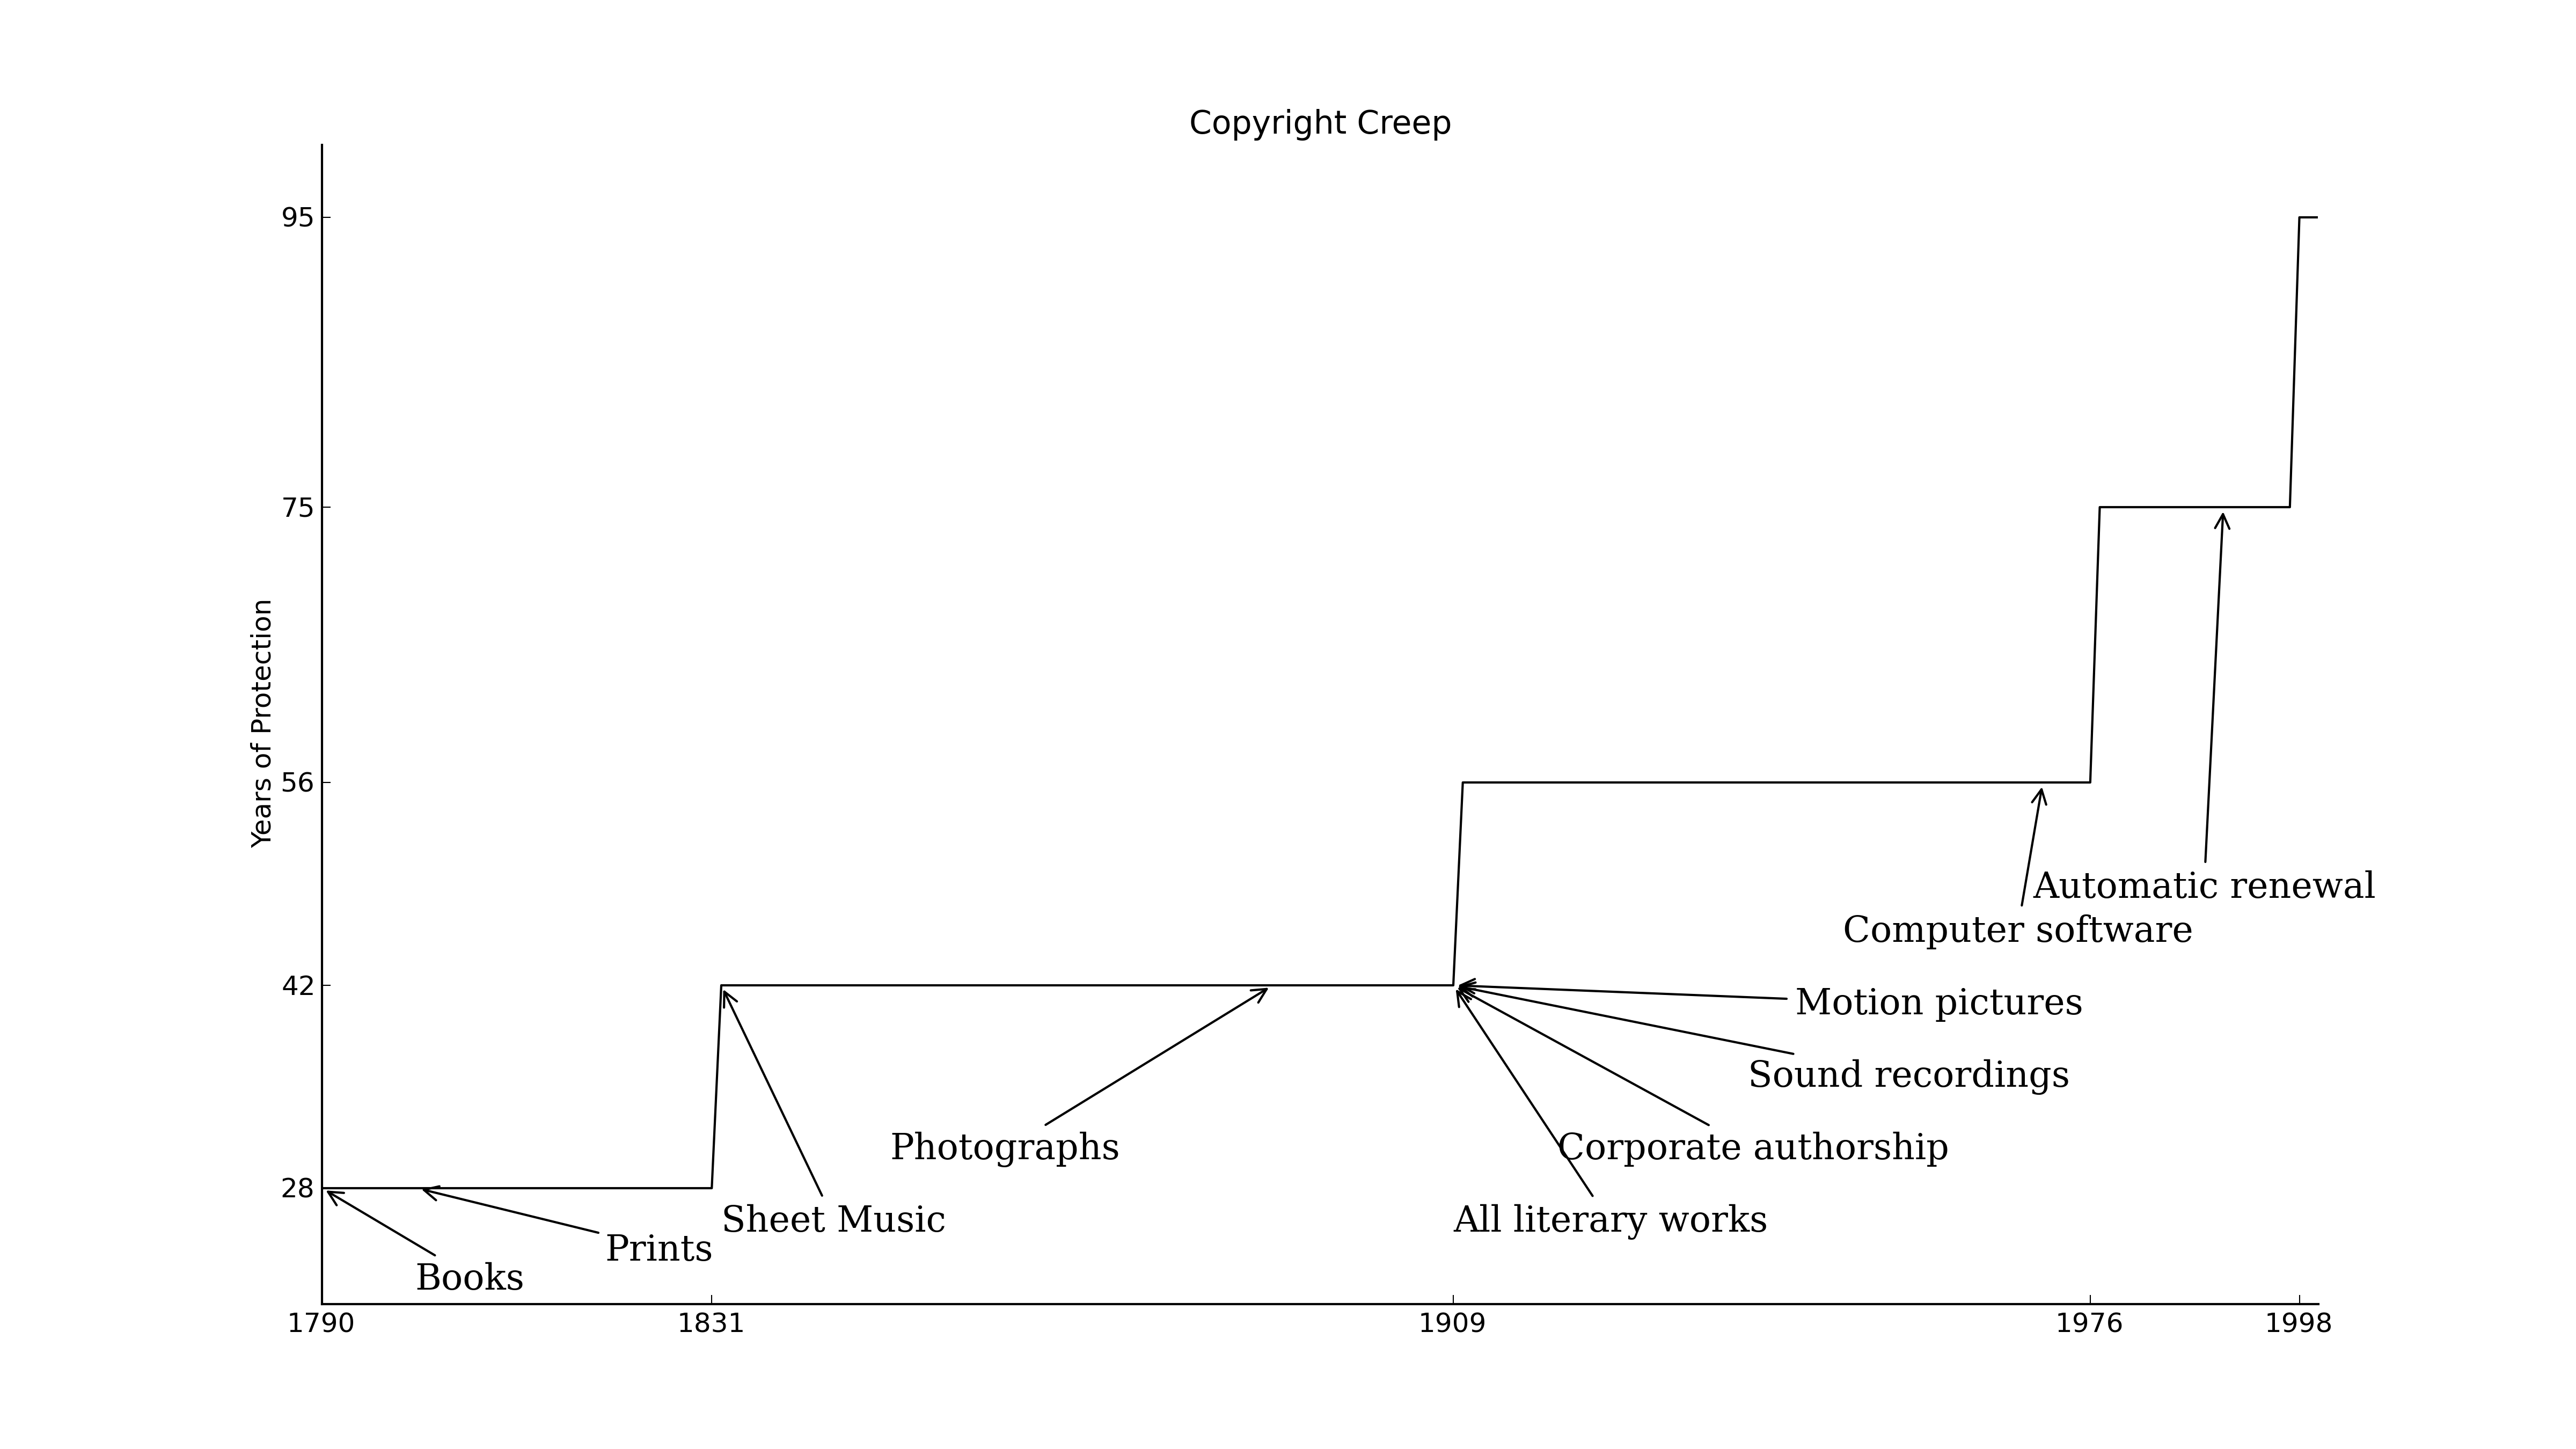
\includegraphics[scale=.275]{copyright_creep.png}
	      \label{fig:copyright_creep}
	  \end{center}
	\end{figure}
\end{frame}

\begin{frame}[t]
    \frametitle{Copyright Term Extension Act}
  \begin{itemize}
    \item<+-> CTEA of 1998
      \begin{itemize}
        \item<+-> Created prior to 1978: 95 year protection.
        \item<+-> Created after 1978: lifetime of the author plus 70 years.
        \item<+-> Challenged on grounds of:
        \begin{itemize}
            \item<+-> The Copyright Clause -- ``limited Times''
            \item<+-> The First Amendment
            \item<+-> The public trust doctrine
        \end{itemize}
        \item<+-> Upheld in \emph{Eldred v. Ashcroft} by SCOTUS (January 15th, 2003).
    \end{itemize}
  \end{itemize}
\end{frame}

\begin{frame}[t]
 \frametitle{Diamond v. Diehr (1981)}
 \begin{itemize}
     \item<+-> Prior to 1981 software was effectively not patentable.
     \item<+-> Mathematical formulas in the abstract are not eligible for patent protection.
     \item<+-> However, a physical machine or process which makes use of a mathematical algorithm is different from an invention which claims the algorithm in the abstract.
     \item<+-> Software is patentable.
 \end{itemize}
\end{frame}

\begin{frame}[t]
    \frametitle{Amazon One-Click Patent}
  \begin{columns}[T]
    \begin{column}{.5\textwidth}
    \begin{block}{}
    \tiny A method and system for placing an order to purchase an item via the Internet. The order is placed by a purchaser at a client system and received by a server system. The server system receives purchaser information including identification of the purchaser, payment information, and shipment information from the client system. The server system then assigns a client identifier to the client system and associates the assigned client identifier with the received purchaser information. The server system sends to the client system the assigned client identifier and an HTML document identifying the item and including an order button. The client system receives and stores the assigned client identifier and receives and displays the HTML document. In response to the selection of the order button, the client system sends to the server system a request to purchase the identified item. The server system receives the request and combines the purchaser information associated with the client identifier of the client system to generate an order to purchase the item in accordance with the billing and shipment information whereby the purchaser effects the ordering of the product by selection of the order button.
    \end{block}
    \end{column}
    \begin{column}{.5\textwidth}
    \begin{block}{}
      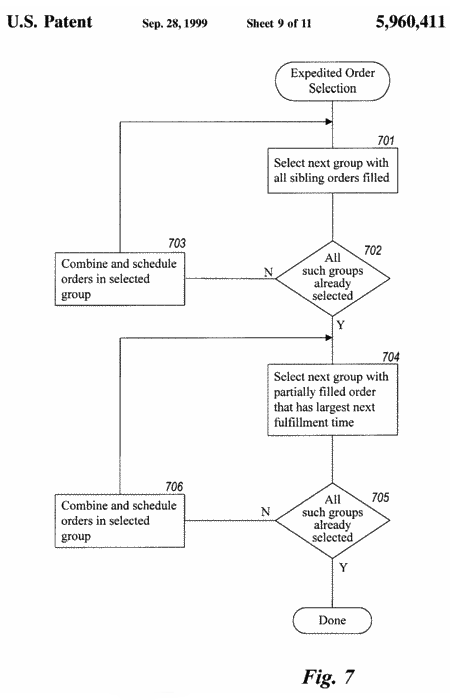
\includegraphics[height=2.75in,angle=0]{Amazon.png}
    \end{block}
    \end{column}
    \end{columns}
\end{frame}


\begin{frame}[t]\frametitle{Growth in Patent Applications} 
\fontsize{6pt}{7.2}\selectfont
\!\!\!\!\!\!\!\!\!\!\!\!\!\!
\begin{figure}[hb]
  \begin{center}
      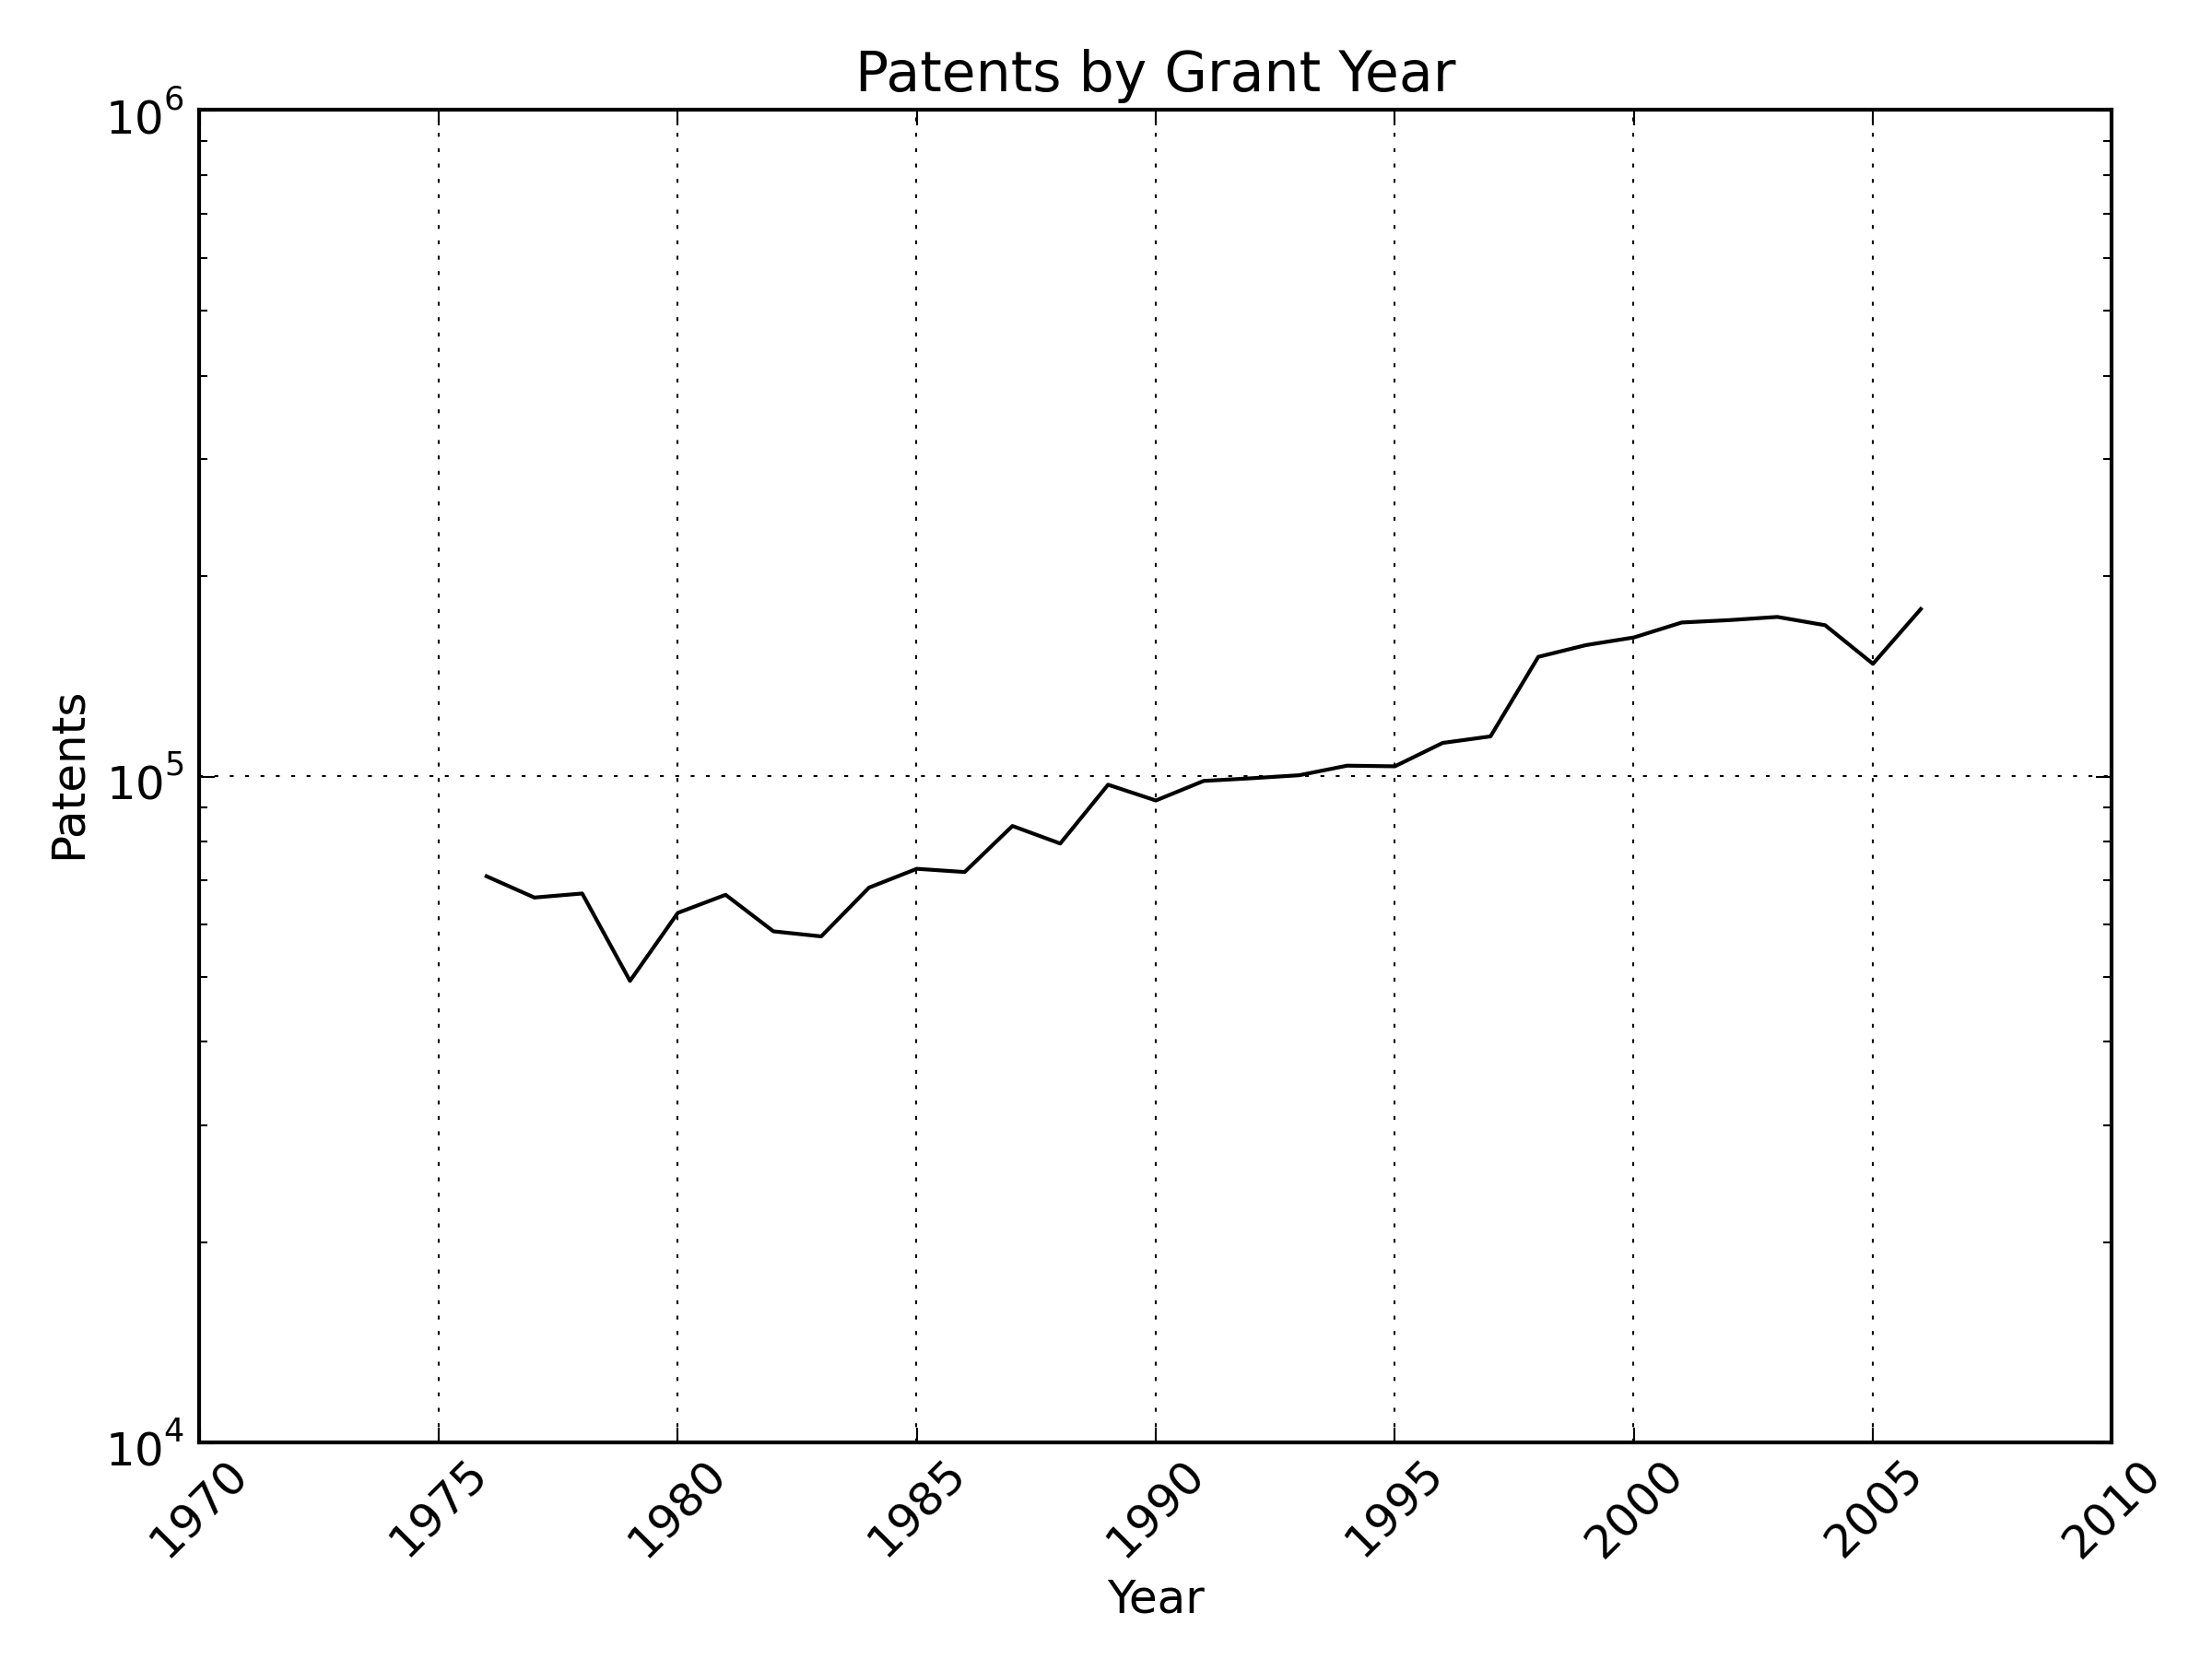
\includegraphics[scale=.5]{grant_year.png}
      \label{fig:grant_year}
  \end{center}
  \!\!\!\!\!
  Hall, et al (2001). ``The NBER Patent Citation Data File''.
\end{figure}
\end{frame}

\begin{frame}[t]\frametitle{Patents by Country} 
\fontsize{6pt}{7.2}\selectfont
\!\!\!\!\!\!\!\!\!\!\!\!\!
\begin{figure}[hb]
  \begin{center}
    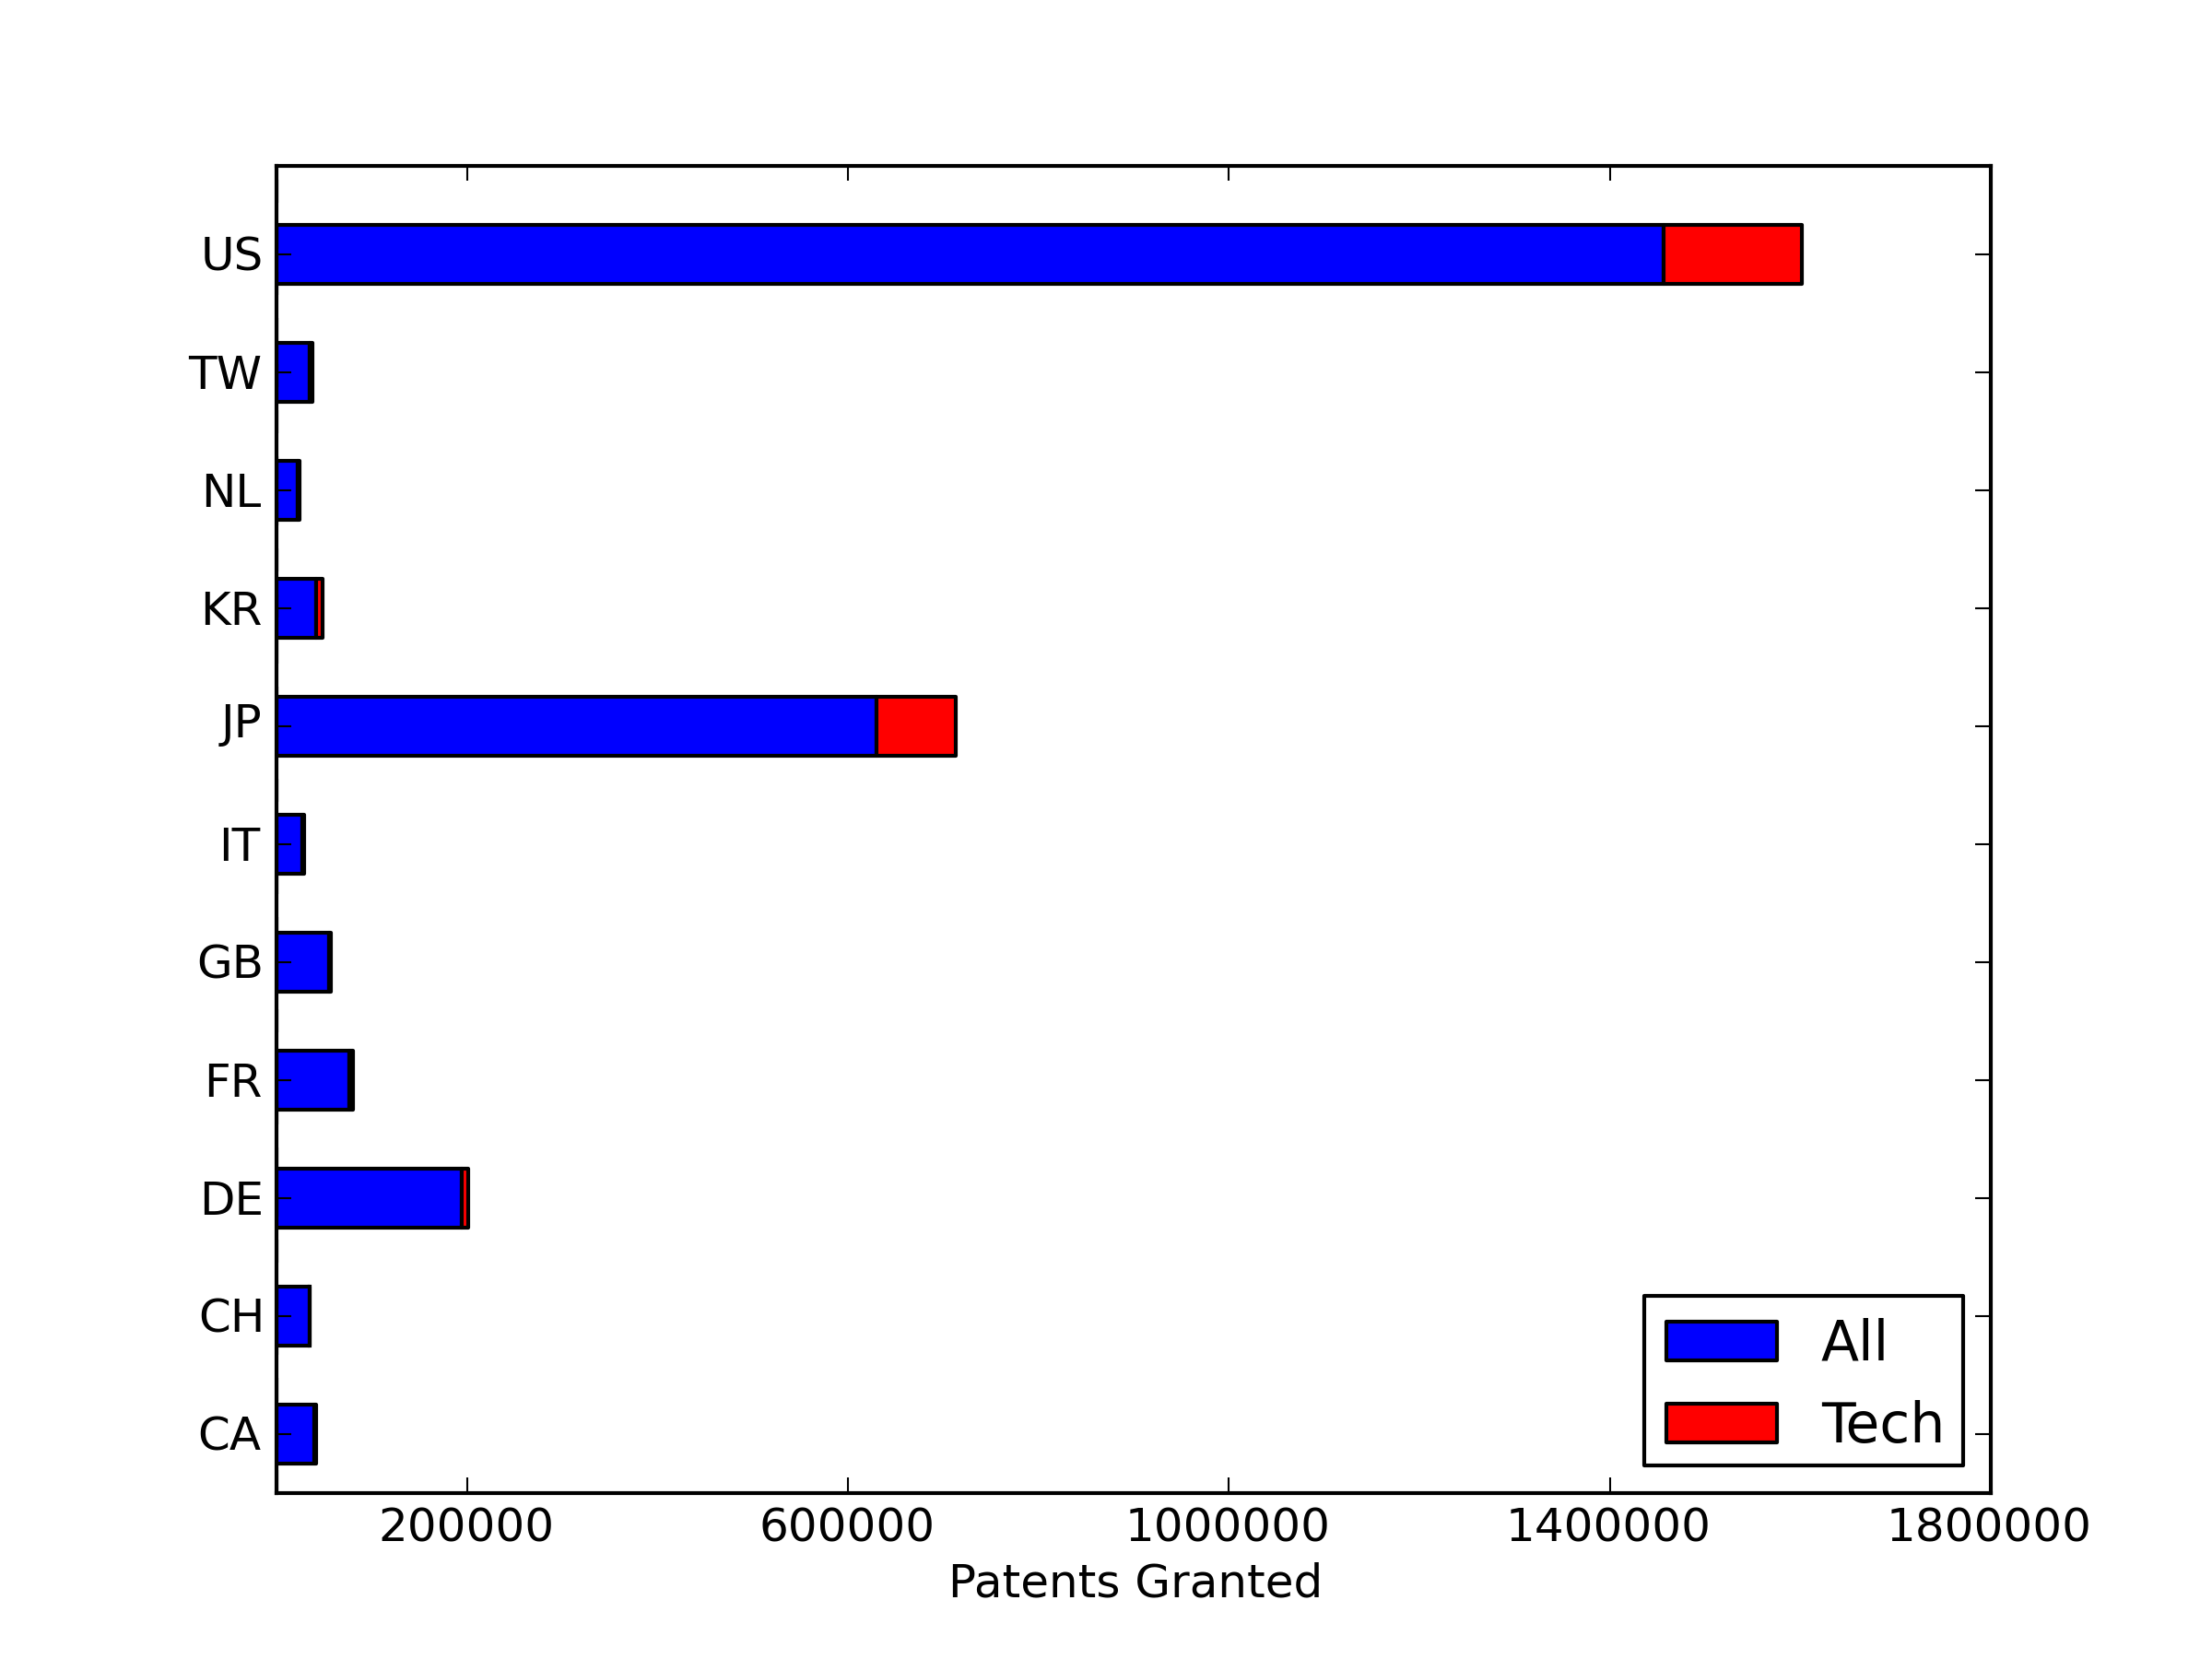
\includegraphics[scale=.5]{by_country.png}
    \label{fig:by_country}
  \end{center}
  \!\!\!\!\!
  Hall, et al (2001). ``The NBER Patent Citation Data File''.  
\end{figure}
\end{frame}

\begin{frame}[t]\frametitle{Patents by Country} 
\fontsize{6pt}{7.2}\selectfont
\!\!\!\!\!\!\!\!\!\!\!\!\!
\begin{figure}[T]
  \begin{center}
    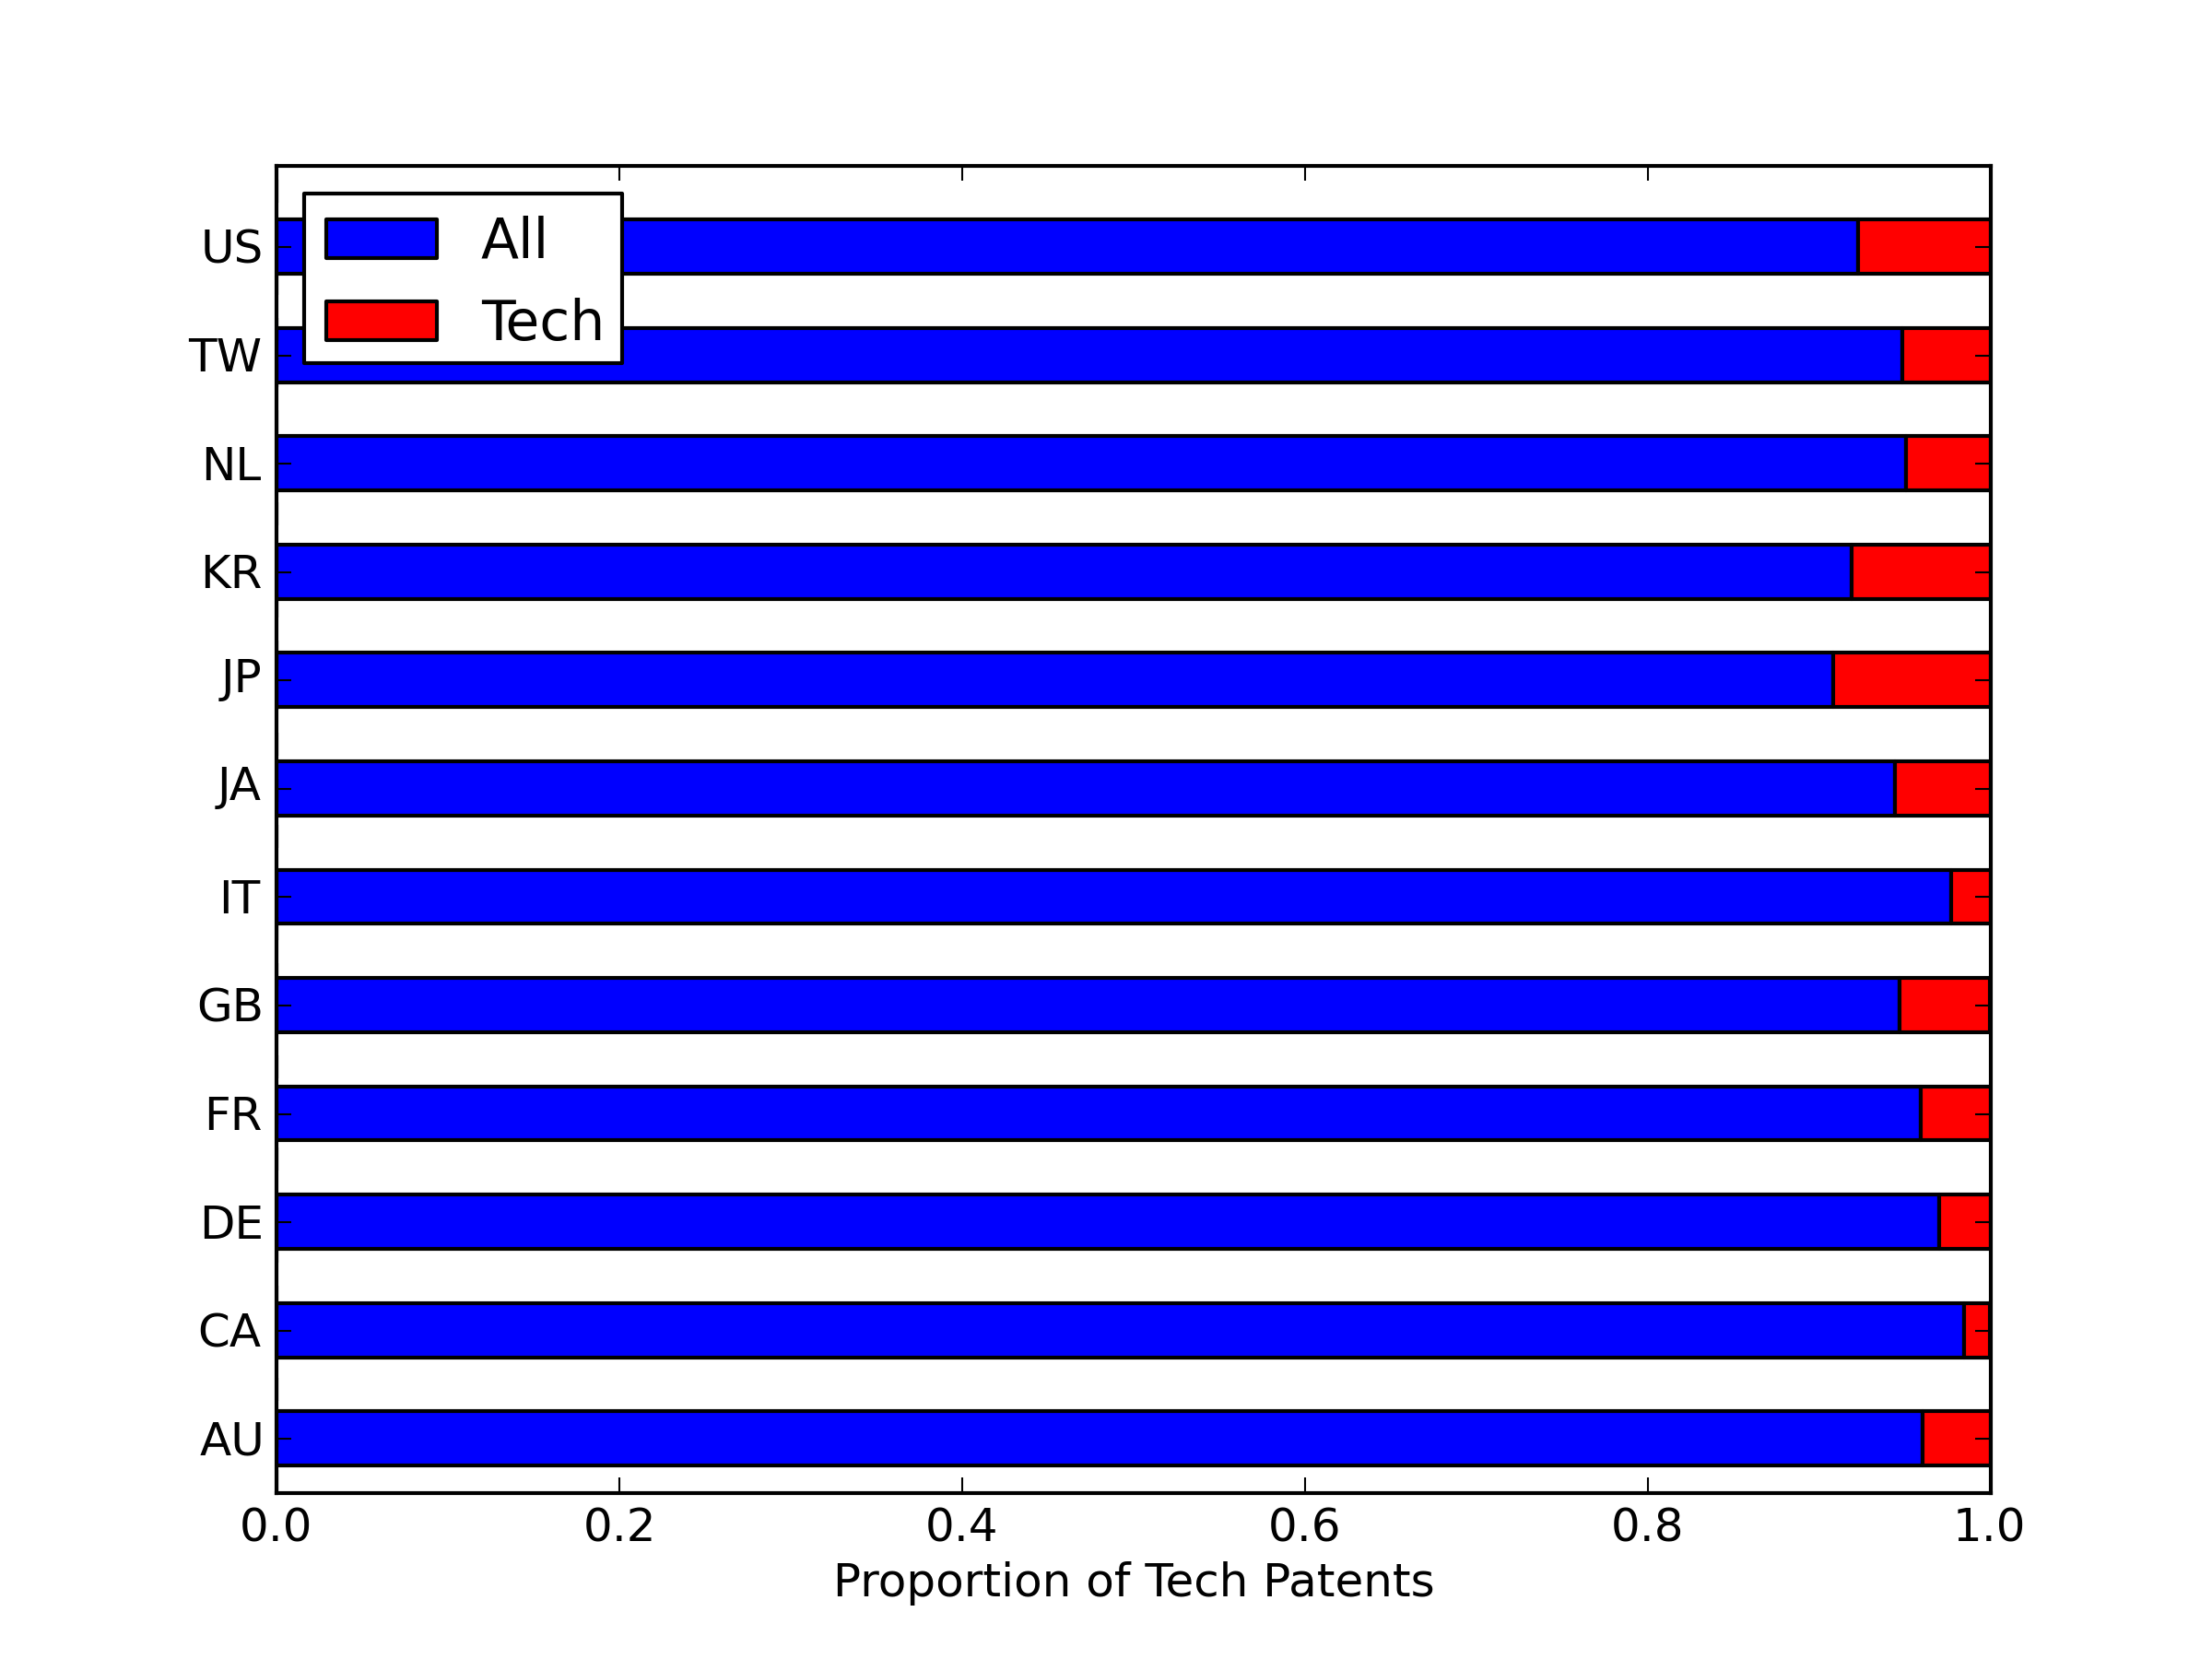
\includegraphics[scale=.5]{by_country_normalized.png}
    \label{fig:by_country_normalized}
  \end{center}
  \!\!\!\!\!
  Hall, et al (2001). ``The NBER Patent Citation Data File''.

\end{figure}
\end{frame}

\begin{frame}[t]\frametitle{Most Cited Patent} 
  \begin{itemize}
    \item<+-> February 2, 1988: Patent No. 4,723,129.
    \item<+-> Bubble jet recording method and apparatus in which a heating element generates bubbles in a liquid flow path to project droplets.
  \end{itemize}
\end{frame}


\begin{frame}[t]\frametitle{Most Cited Patent} 
  \begin{itemize}
    \item February 2, 1988: Patent No. 4,723,129.
    \item Bubble jet recording method and apparatus in which a heating element generates bubbles in a liquid flow path to project droplets.
    \item Canon Ink Jet printers.
  \end{itemize}
\end{frame}

\begin{frame}[t]
  \frametitle{Why does open source coexist?}
  \begin{itemize}
    \item<+-> Control over product performance.
    \item<+-> Hobbyists and enthusiasts.
    \item<+-> Display of skill or resume padding.
    \begin{itemize}
        \item<+-> Hann et. al (2004)
    \end{itemize}
    \item<+-> Competitive rents (Boldrin \& Levine).
    \begin{itemize}
        \item<+-> Which model version fits?
        \item<+-> What can we say about the implications?
    \end{itemize}
  \end{itemize}
\end{frame}

\begin{frame}[t]
  \begin{quotation}
    The evidence (and the common sense of anyone involved with OS software) shows   that the source of competitive rents is the complementary sale of expertise.
  \end{quotation}
  \begin{quotation}
      ...only small rents can be obtained through the sale of copies. [Purchasers] also have a demand for services, ranging from support and consulting to customization. They naturally prefer to hire the creators of the programs who in the process of writing the software have developed specialized expertise that is not easily matched by imitators.
  \end{quotation}
  - Boldrin \& Levine (2009)
\end{frame}


\section{Boldrin and Levine (2002)}
\label{sec:boldrin_and_levine_2002}

\begin{frame}
  \frametitle{Boldrin \& Levine}
  Boldrin \& Levine: alternate notation\\
  \begin{table}[ht]
    \caption{Alternate Notation}
    \centering
  \begin{tabular}{c c c}
    \hline\hline
      BL &  & New\\ [0.5ex] 
    \hline
    $\delta$ & $\longrightarrow$ & $\beta$  \\ 
    $\beta$ & $\longrightarrow$ & $\lambda$ \\
    $\zeta$ & $\longrightarrow$ & $1 - \delta$ \\[1ex] 
    \hline
   \end{tabular}
   \label{table:altnot}
  \end{table}
\end{frame}

\begin{frame}[t]
  \frametitle{Boldrin \& Levine: General Model Revisited}
  \begin{itemize}
    \item<+-> Distinguish between productive input and consumption good: $\{k,c\}$.
    \item<+-> $c_t = F(k_t^c,l_t^c)$, $x_t = G(k_t^k,l_t^k)$.
  \end{itemize}
\end{frame}

\begin{frame}[t]
  \frametitle{Boldrin \& Levine: General Model Revisited}
  \begin{itemize}
	  \item<+-> Agent solves $\sum_{t=0}^\infty\beta^t[u(c_t)-wL_t]$:
	  \begin{itemize}
        \item<+-> $\lambda k_t$ units available tomorrow: $k_{t+1} = \lambda k_t + x_t$.
	    \item<+-> $\lambda > 1$ gives us the $24/7$ case.
	  \end{itemize}
  \end{itemize}
\end{frame}

\begin{frame}[t]\frametitle{Boldrin \& Levine: General Model Revisited}
    \begin{columns}[T]
      \begin{column}{.6\textwidth}
        \begin{minipage}[c][.35\textheight][c]{\linewidth}
        \begin{itemize}
          \item<+-> Given $\{k_t, x_t, L_t\}$, the solution $c_t = T(k_t,x_t,L_t)$ traces a production possibility frontier\\
        \end{itemize}
        \end{minipage}
    \end{column}
    \begin{column}{.45\textwidth}
      \begin{minipage}[c][.4\textheight][c]{\linewidth}
        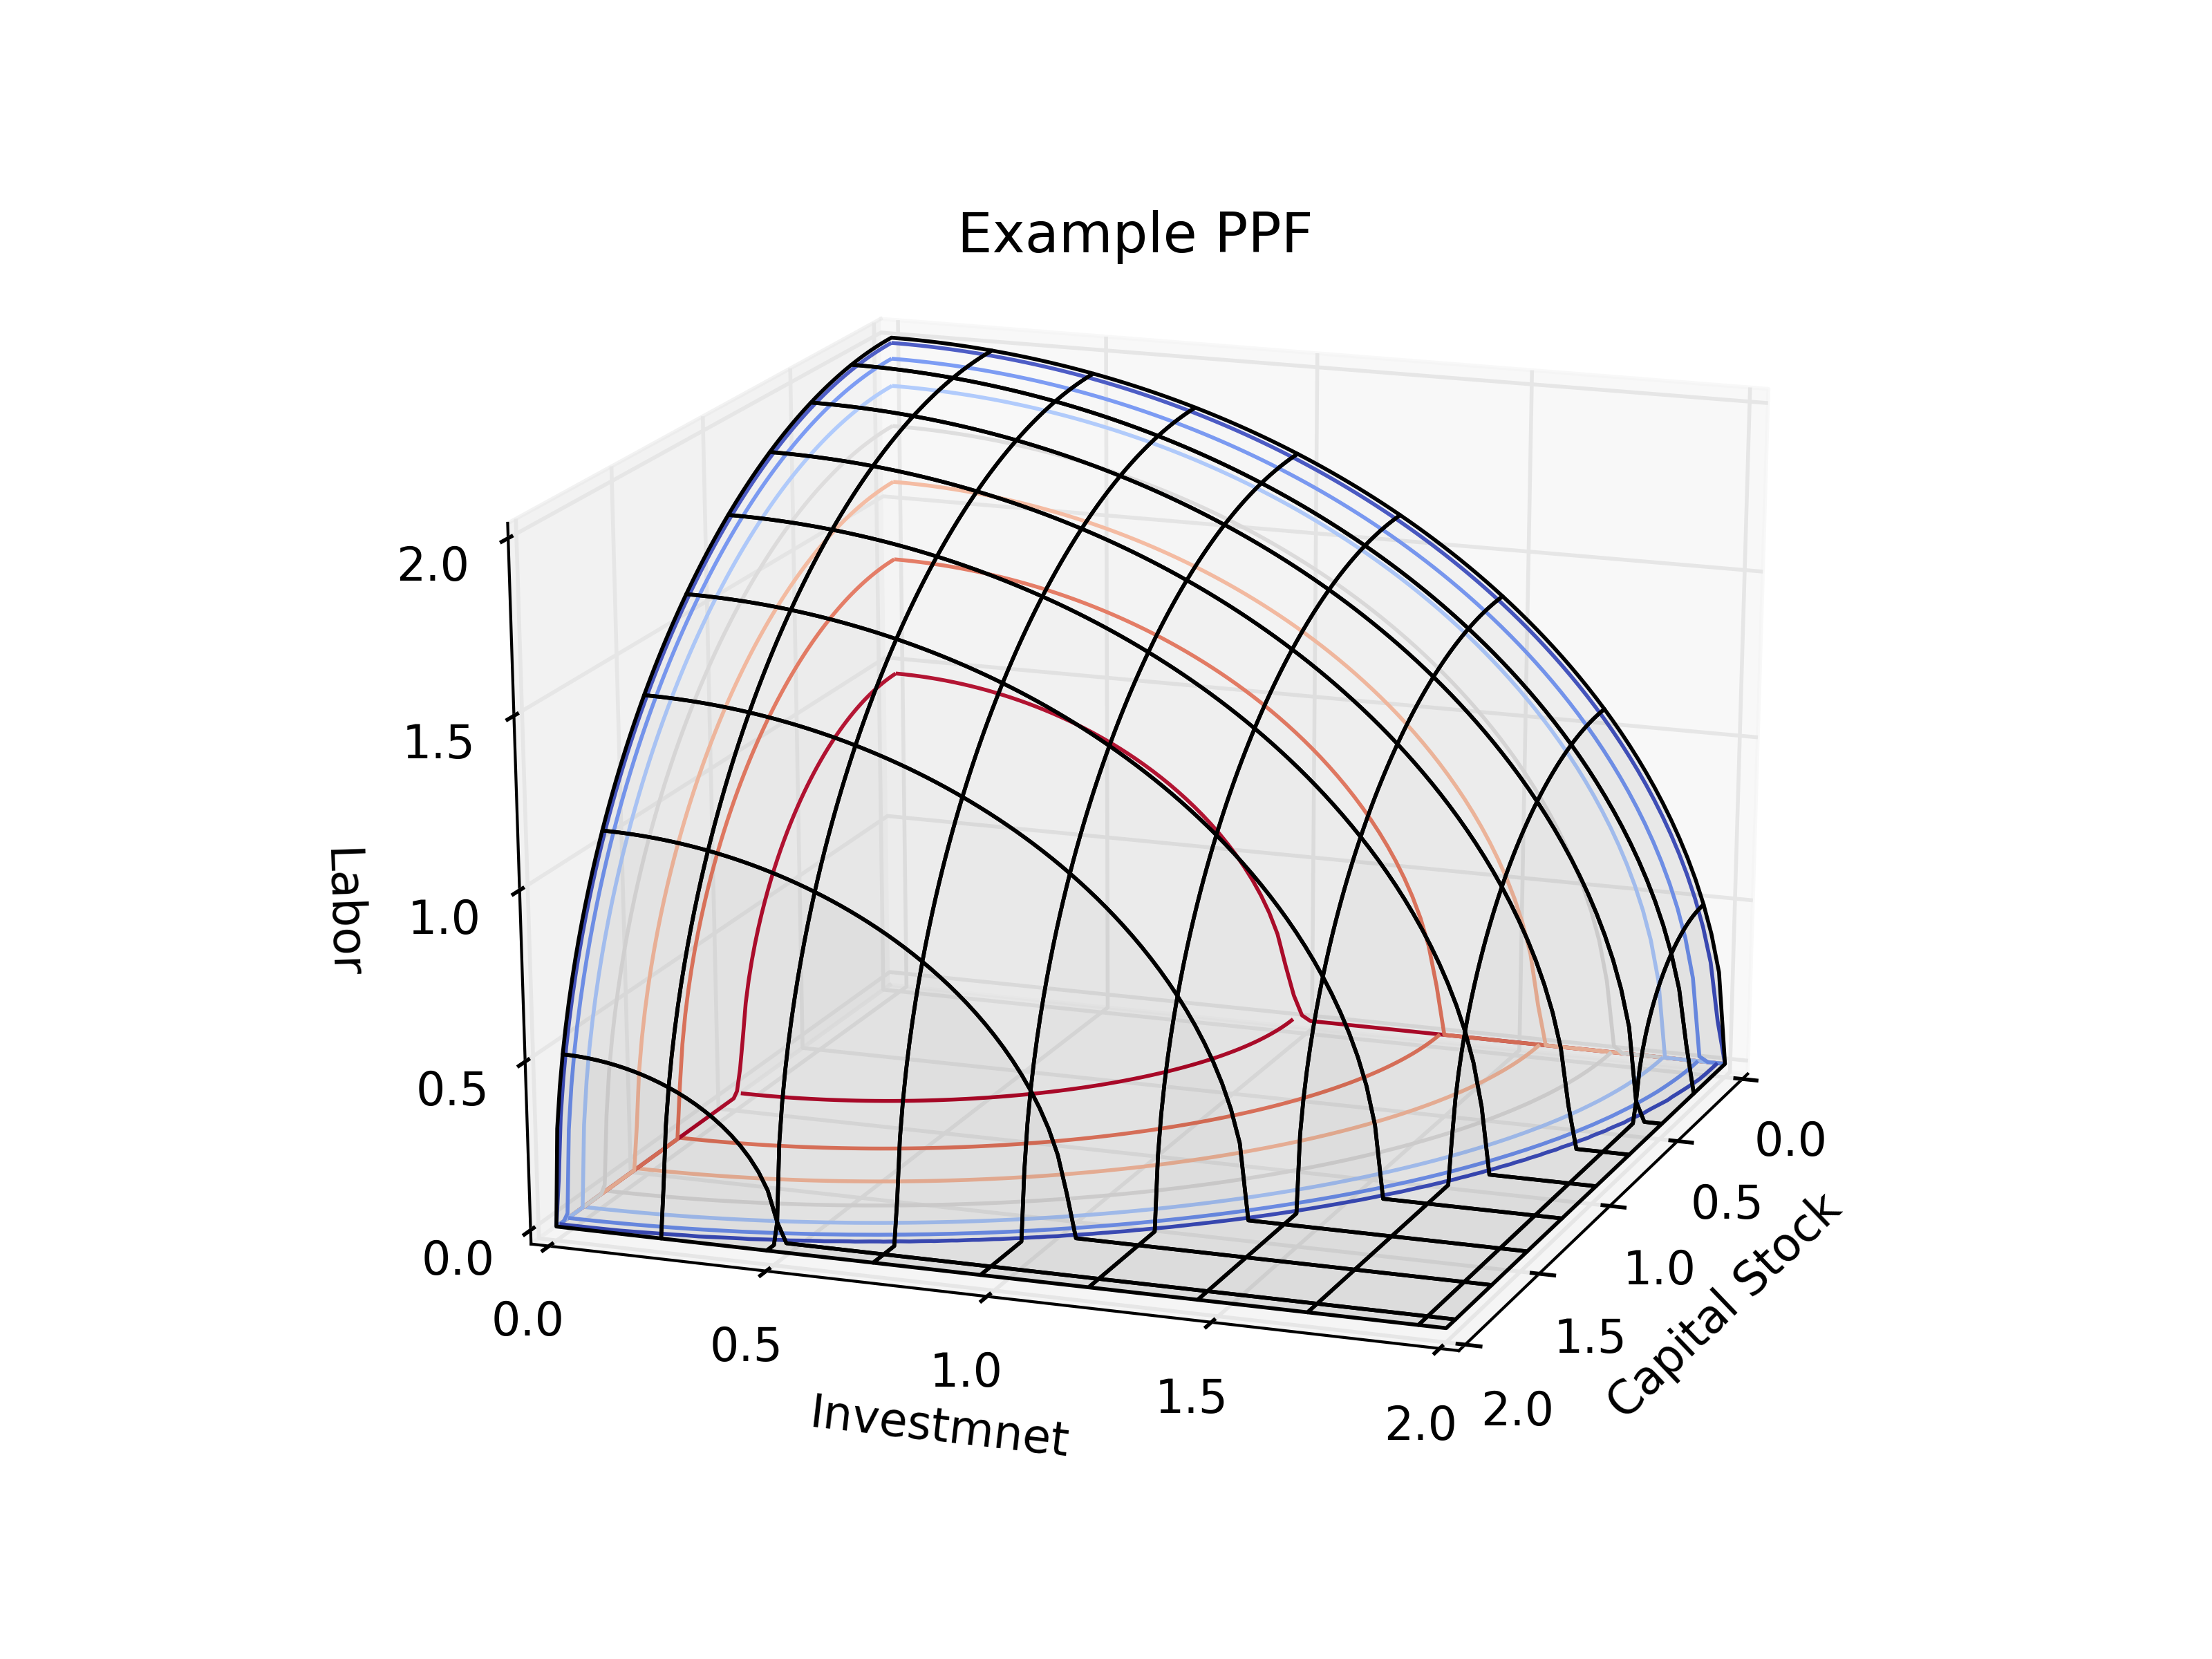
\includegraphics[scale=.30]{example_ppf_contour.png}
          \label{fig:ppf}
        \end{minipage}
    \end{column}
  \end{columns}

  \begin{minipage}[c][.3\textheight][c]{\linewidth}
  \begin{itemize}
    \item<+-> $L_t$ solves $\underset{L_t}{max}$ $u[T(k_t,x_t,L_t)]-wL_t$
    \item<+-> The problem restated:
      \begin{align*}
        &\nu(k_0)=
        \max_{\{k_t\}_{t=1}^\infty} \sum_{t=0}^\infty\beta^tV(k_t,k_{t+1} - \lambda k_t)
          \hspace{13mm}\\
        &s.t. \ \ \ \ \ \ \lambda k_t + \overline{x}(k_t) \ge k_{t+1} \ge \lambda k_t
      \end{align*}
  \item<+-> As before, $q_0 = \nu ' (k_0) > 0$ yields positive competitive rents
  \end{itemize}
  \end{minipage}
\end{frame}

\begin{frame}[t]
  \frametitle{Open source innovation and selling expertise}
  \begin{itemize}
    \item<+-> Investment: $x_t = G(L_t)$\\ (labor is chosen according to $L_t = g(x_t)$)
    \item<+-> Consumption (services): $c_t = f(h_t)$
    \item<+-> The innovator starts with $h_0$
    \begin{itemize}
      \item<+-> As soon as this occurs, others can begin accumulating productive capacity (expertise in the software)
      \item<+-> $h_{t+1} = x_t + (1-\delta)*h_t$
    \end{itemize}
  \end{itemize}
\end{frame}

\begin{frame}[t]\frametitle{Open source innovation and selling expertise}
  \begin{itemize}
    \item<+-> Consumer utility same as the general case
    \item<+-> Planners Problem:\\ 
    \begin{centering}
      $\nu(h_t) = \underset{x_t \ge 0}{max} \{u(c_t) - wg(x_t) + \beta\nu(h_{t+1})\}$
    \end{centering}
    \item<+-> First order condition:\\
    \begin{centering}
      $wg'(x_t) = \beta\nu'(h_{t+1})$
    \end{centering}
    \item<+-> This can be decentralized with prices $\{p_t, q_t\}$ for services and capital
    \begin{itemize}
    \item<+-> $p_t = u'(c_t)$
    \item<+-> $q_t = \nu'(h_t) = u'(c_t)f'(h_t) + \beta(1-\delta)\nu'(h_{t+1})$ 
    \end{itemize} 
  \end{itemize}
\end{frame}

\begin{frame}[t]\frametitle{Open source innovation and selling expertise}
  \begin{itemize}
    \item<+-> Rearranging:
    \begin{equation*}
       q_0 = \sum_{t=0}^\infty(\beta(1-\delta))^tu'(c_t)f'(c_t)
    \end{equation*}
     \item<+-> The open source innovation is viable as long as $q_0k_0 > C$
     \item<+-> Perhaps more elucidating:\\
	 \begin{equation*}
     q_0 = \underbrace{u'(c_0)f'(h_0)}_{\text{\color{red}first mover advantage}} +\ \ \underbrace{(1-\delta)wg'(x_0)}_{\text{\color{red}cost of imitation}} 
	 \end{equation*} 
  \end{itemize}
\end{frame}

\begin{frame}[t]\frametitle{Conclusion}
  \vspace{20mm}
  \begin{itemize}
    \item<+-> Competitive rents can explain the open source phenomenon.
	\item<+-> Innovation occurs without the excludability of ideas.
	\item<+-> Particularly fatal to the notion that monopolies must exist for innovation.
  \end{itemize}
\end{frame}

\section{Acemoglu and Akcigit (2012)}
\label{sec:acemoglu_and_akcigit_2012}

\subsection{Introduction}
\label{sub:introduction}

\begin{frame}[t]\frametitle{Intro}
  \begin{itemize}
    \item<+-> Daron Acemoglu and Ufuk Akcigit (2012) - Intellectual Property Rights Policy, Competition And Innovation.
    \item<+-> Optimal \emph{state-dependent} Intellectual Property Rights policy in a dynamic environment.
    \item<+-> IPR depends on technology gap in an industry (state-dependence).
    \item<+-> Standard tradeoff between monopoly distortions and motivation.
    \item<+-> Novel motivation for leaders.
  \end{itemize}
\end{frame}

\subsection{Literature Review}
\label{sub:literature_review}
\begin{frame}[t]\frametitle{Previous Research} 
  \begin{itemize}
    \item<+-> \emph{Static} tradeoff between R\&D incentive and monopoly distortions. Mixed conclusions.
    \item<+-> Mechanism design approach.  Menu of patents and fees.
    \item<+-> Step-by-step innovation (Aghion, Harris, and Vickers 1997) --- Higher growth from stiffer competition.
    %\item<+-> Look for predecessors of state-dependent IPR.  They claim to ``explicitly introduce'' it.
    %\item<+-> Look for predecessor of dynamic effects, not just static R\&D incentives / monopoly rents tradeoff.
    %\item<+-> Par. 3 pg. 5 notes some mechanism-design papers that might be worth skimming for previous research.
  \end{itemize}
\end{frame}

% \subsection{Contributions}
% \label{sub:contributions}

% \begin{frame}[t]\frametitle{New Contributions} 
%   \begin{itemize}
%     \item<+-> State-dependent IPR.
%     \item<+-> Slow catch-up, compulsory licensing %(check on this).
%     \item<+-> Full GE model % (probably done before, but first in the Aghion et. al line?)
%   \end{itemize}
% \end{frame}

\subsection{Preferences}
\label{sub:preferences}

\begin{frame}[t]\frametitle{Consumers' Preferences} 
  \begin{itemize}
    \item<+-> Single final good.  Continuum of 1 individuals.
      \begin{equation*} \label{eq:pref}
        \mathbb{E}_t \int_t^\infty exp(-\rho(s - t))\mathrm{ln}\,   C(s)ds
      \end{equation*}
      where $\rho$ is the discount factor.
      
  \item<+-> Supply 1 unit of labor.
  \item<+-> Own balanced portfolio of intermediate goods producers.
  \end{itemize}
\end{frame}

\subsection{Production}
\label{sub:production}

\begin{frame}[t]\frametitle{Technology-Final Good} 
  \begin{itemize}
    \item<+-> Output of final good: $Y(t) = C(t)$.
    
    \item<+-> Production of $Y(t)$:
      \begin{equation*} \label{eq:tech_output}
        % Why log output? Cobb-Douglas since log of products is sum
        % i.e. the integral?  CD need not be HOD 1.
        \ln Y(t) = \int_{0}^{1} \ln y(j, t) d\,j 
      \end{equation*}
      where $y(j, t)$ is the quantity of intermediate good $j$ used.
    \item<+-> Perfect substitutes between intermediate varieties.
    
    %% Is this the right place for EE?
    % \item<+-> Euler Equation:
    %   \begin{equation*}
    %     g(t) \equiv \frac{\dot{C}(t)}{C(t)} = \frac{\dot{Y}(t)}{Y(t)} = r(t) - \rho
    %   \end{equation*}
  \end{itemize}
\end{frame}

\begin{frame}[t]\frametitle{Technology-Intermediate Good} 
  \begin{itemize}
    \item<+-> Each industry $j \in [0, 1]$ has two firms. Firms denoted by $i$ (leader) and $-i$ (follower).

    \item<+-> Output:
      \begin{equation*} \label{eq:intermediate_production}
        y(j, t) = q_i(j, t)l_i(j, t)
      \end{equation*}
      where $q_i$ is a technology level and $l_i$ is labor used. 

    \item<+-> Limit pricing:
      \begin{equation*} \label{eq:limit_pricing}
        p(j, t) = \frac{w(t)}{q_{-i}(j, t)}      
      \end{equation*}

    \item<+-> Cobb-Douglas production of final good implies:
    %  TODO: Verify this.
      \begin{equation*}
        y(j, t) = \frac{q_{-i}(j, t)}{w(t)}Y(t)
      \end{equation*}
  \end{itemize}
\end{frame}

\begin{frame}[t]\frametitle{Technology-Innovation} 
  \begin{itemize}
    \item<+-> Poisson Innovation:
      \begin{equation*} \label{eq:tech_rd_technology}
        x_i(j, t) = F(h_i(j, t))
      \end{equation*}
      where $h_i(j, t)$ is the number of workers in R\&D.
      Also define $G(x_i(j,t)) \equiv F^{-1}(x_i(j,t))$ (R\&D employment).
    \item<+-> Leader innovation: technology $\uparrow$ by factor $\lambda > 1$.
    \item<+-> Follower innovation: quick catch-up (not patent infringing).
    \item<+-> Technology levels are ladder rungs: $q_i(j, t) = \lambda^{n_{ij}(t)}$, with $n_{ij}(t)$ giving the rung for firm $i$ in industry $j$.
    \item<+-> Technology gap: $n_j(t) = n_{ij}(t) - n_{-ij}(t)$
  \end{itemize}
\end{frame}

\subsection{Patent Policy}
\label{sub:patent_policy}

\begin{frame}[t]\frametitle{Patent Policy}
  \begin{itemize}
    \item<+-> Patents expire at Poisson rate: $\eta_{n_j}(t)$.
    \item<+-> Law of motion for technology gap in industry $j$:
      \begin{equation*} \label{eq:tech_law_of_motion}
        \eta_j(t + \Delta t) =
        \begin{cases}
          \eta_j(t) + 1 & \textrm{prob } x_i(j,t)\Delta t + o(\Delta t)\\
          0 & \textrm{prob } x_{-i}(j,t)\Delta t + \eta_{n_{j(t)}}\Delta t + o(\Delta t) \\
          \eta_j(t) & \textrm{with the remainder} 
        \end{cases}
      \end{equation*}
  \item<+-> Write the patent policy as $\bm{\eta} : \mathbb{N} \rightarrow \mathbb{R}$.
  \end{itemize}
\end{frame}

% \subsection{Profits}
% \label{sub:profits}



\subsection{Equilibrium}
\label{sub:equilibrium}
\begin{frame}[t]\frametitle{Equilibrium} 
  \begin{itemize}

  \item<+-> $\bm{\mu}(t) \equiv {\mu_n(t)}_{n=0}^\infty$ is a distribution of \emph{industries} over \emph{technology gaps}.
  
  \item<+-> Loosely define an \textsc{Allocation} as a sequence of decisions for leaders and followers, sequence of wage rates, and a sequence of distributions over gaps.

  \item<+-> Loosely define an \textsc{Equilibrium} as a sequence of decisions, wages, and output such that markets clear, firms' expected profits are maximized, and R\&D policies are best responses. 

  \end{itemize}
\end{frame}


\begin{frame}[t]\frametitle{Labor Market} 
  \begin{itemize}
    \item<+-> Three sources of demand: Production of intermediaries, and R\&D by each firm.
    \item<+-> Combine the demand for intermediates: $y(j, t) = \frac{q_{-i}(j, t)}{w(t)}Y(t)$ with the production function to get:

      \begin{equation*}
        l_n(t) = \frac{\lambda^{-n}Y(t)}{w(t)}
      \end{equation*}
    and so
      \begin{equation*} \label{eq:labor_clearing}
        1 \geq \sum_{n=0}^{\infty} \mu_n(t) \Big[\frac{1}{\omega(t)\lambda^n} + G(x_n(t))    + G(x_{-n}(t))\Big]
      \end{equation*}
      where $\omega(t)$ is labor's share of income.

  \end{itemize}
\end{frame}
\subsection{Steady State}
\label{sub:steady_state}
\begin{frame}[t]\frametitle{Firm's Value Function} 
  \begin{itemize}
    \item<+-> Net present value when leading by $n$:
      \begin{equation*}
        V_n(t) = \mathbb{E}_t \int_{t}^{\infty} exp(-r(s - t))[\Pi(s) - w(s)G(\hat{x}(s))]\,ds 
      \end{equation*}
    \item<+-> ``Normalized''value function ($v_n(t) = V_n(t) / Y(t)$):
      \begin{equation*} \label{eq:rvf_leader}  % rvf: recursive value function
          pv_n = \max_{x_n \geq 0}\ \ (1 - \lambda^{-n}) - \omega^*G(x_n) + x_n[v_{n+1} - v_n] + [x_{-n}^* + \eta_n][v_0 - v_n]
        \end{equation*}
    \item<+-> Instantaneous operating profits: $(1 - \lambda^{-n})$.
    \item<+-> R\&D costs: $\omega^*(t)G(x_n(t))$.
    \item<+-> With probability $x_n(t)$ you innovate.
    \item<+-> With probability $x_{-n}^*(t) + \eta_n$ he innovates or your patent expires.
  \end{itemize}
\end{frame}

\begin{frame}[t]\frametitle{Firm's Value Function} 
  \begin{itemize}
    \item<+-> Tied firm's value function:
      \begin{equation*} \label{eq:rvf_tied}
        \rho v_0 = \max_{x_0 \geq 0} -\omega^*G(x_{0}) + x_{0}[v_1 - v_0] + x_0^*[v_{1} - v_0]
      \end{equation*}

    \item<+-> Follower's value function:
      \begin{equation*} \label{eq:rvf_follower}
        \rho v_{-n} = \max_{x_{-n} \geq 0} -\omega^*G(x_{-n}) + [x_{-n} + \eta_n][v_0 - v_{-n}] + x_n^*[v_{-n-1} - v_{-n}])
      \end{equation*}
  \end{itemize}
\end{frame}

\begin{frame}[t]\frametitle{Optimal R\&D}
  \!\!\!\!\!\!\!\!\!\!\!\! % Move it up.
  \begin{align} \label{eq:ss_rd_policies}
    &x_n^*    = max \big\{G'^{-1}\Bigg(\frac{[v_{n+1} - v_n]}{\omega^*}\Bigg)   ,0\}\\
    &x_{-n}^* = max \big\{G'^{-1}\Bigg(\frac{[v_0  - v_{-n}]}{\omega^*}\Bigg)   ,0\}\\
    &x_0^*    = max \big\{G'^{-1}\Bigg(\frac{[v_1     - v_0]}{\omega^*}\Bigg)   ,0\}
  \end{align}

  Say patent protection weakens for $n + 1$:
  \begin{itemize}
    \item<2-> Disincentive Effect: $\downarrow v_{n+1} \Rightarrow \downarrow v_{n+1} - v_n \Rightarrow \downarrow x_n^*$.
    \item<3-> Incentive Effect: $\downarrow v_{n+1} \Rightarrow \uparrow v_{n+2} - v_{n+1} \Rightarrow \uparrow x_{n+1}^*$.
    \item<4-> Composition Effect: $x_n$ is decreasing in $n$. More firms in close competition. Higher aggregate R\&D.
    \item<5-> Level Effect: Reduce prices and markups.  Less duplicative R\&D.
  \end{itemize}
\end{frame}

\subsection{Results}
\label{sub:results}
\begin{frame}[t]\frametitle{Uniform Policy} 
Problem is identical for all followers.

Given some assumptions (positive R\&D, non-zero profits) \ldots
\begin{itemize}
  \item<+-> $v_{-1} \leq v_0$; $\{v_n\}_{n=0}^{\infty}$ is bounded and strictly increasing.
  \item<+-> $x_0^* > x_1^*, x_0^* \geq x_{-1}^*$, and $x_{n+1}^* \leq x_n^*\ \forall n \in \mathbb{N}$.
  \item<2> Tied firms innovate the most.
  \item<2> Past that innovation is decreasing in the gap.
\end{itemize}
\end{frame}

\subsection{Optimal IPR}
\label{sub:optimal_ipr}
\subsection{Benchmark: Full IPR}
\label{sub:benchmark_full_ipr}
\begin{frame}[t]\frametitle{Optimal Uniform IPR} 
  \begin{itemize}
    \item<+-> Turns out that if $\eta_n = \eta \ \forall n$, $\eta^* = 0$ (Patents never expire).
    \item<+-> Positive composition effect (more firms in close competition) overwhelmed by negative disincentive effect.
  \end{itemize}
\end{frame}

\begin{frame}[t]\frametitle{Optimal State-Dependent IPR} 
  \begin{itemize}
    \item<+-> Growth rate increases from 1.86\% to 2.04\%.
    \item<+-> Optimal patent length is increasing in technology gap. 
  \end{itemize}
\end{frame}

\begin{frame}[t]\frametitle{Full IPR} 
  \begin{center}
    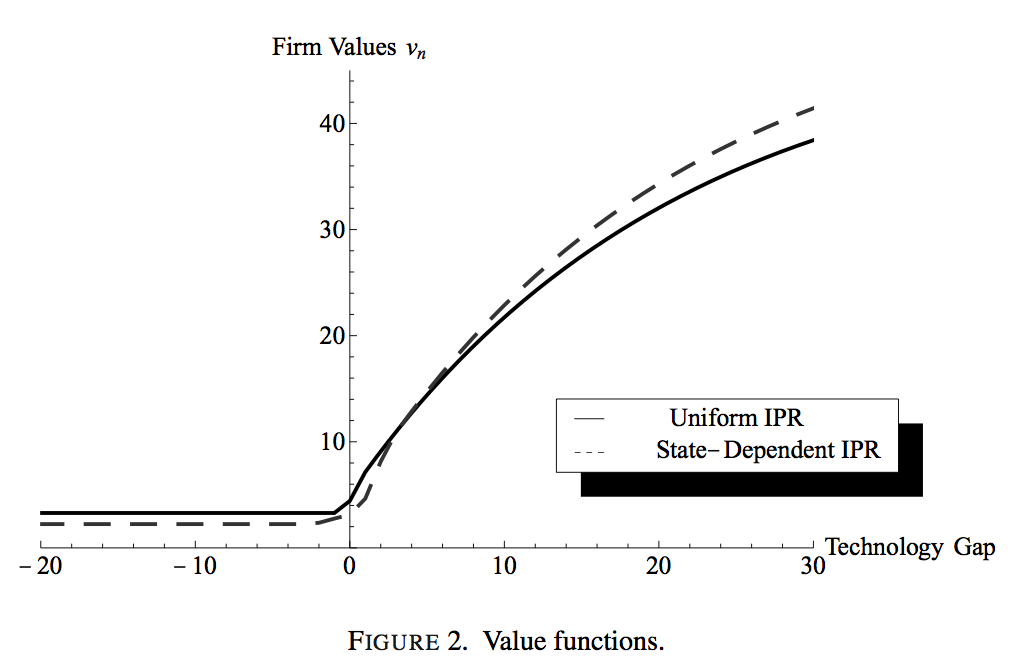
\includegraphics[scale=.31]{full_ipr_value.png}
    \label{fig:full_ipr_value}
  \end{center}
\end{frame}

\begin{frame}[t]\frametitle{Full IPR} 
  \begin{center}
    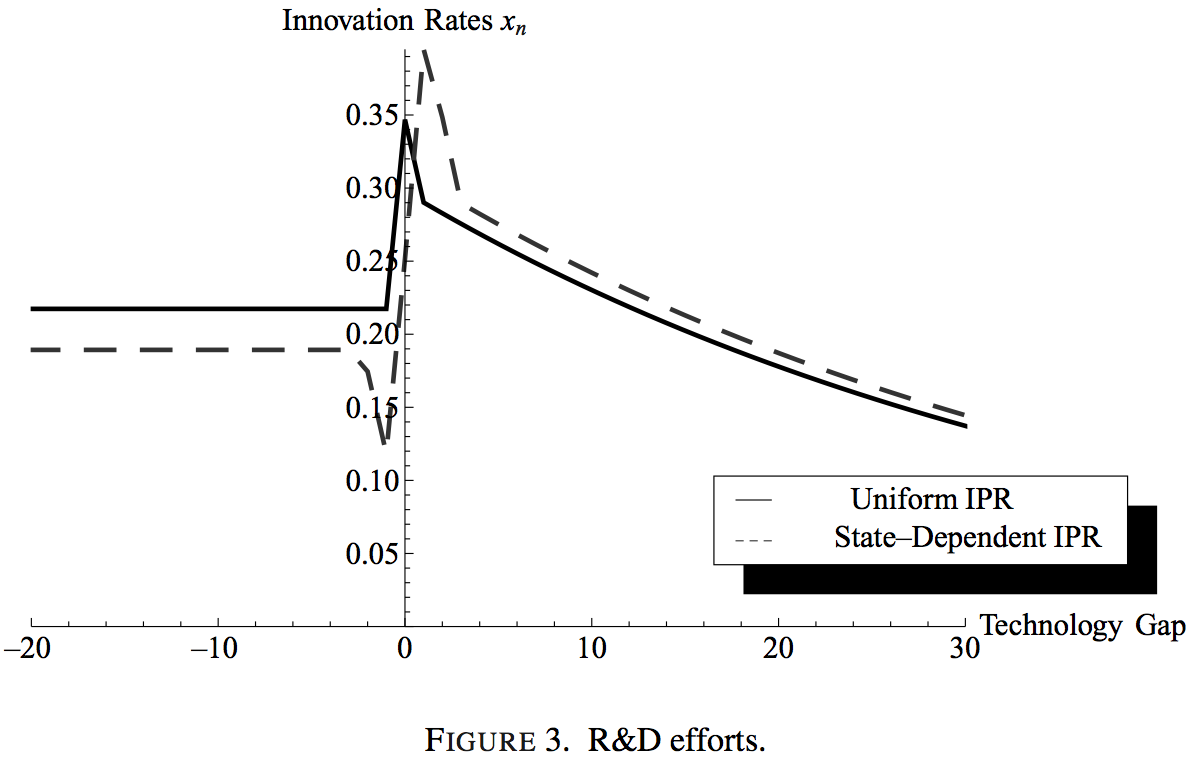
\includegraphics[scale=.28]{full_ipr_rnd.png}
    \label{fig:full_ipr_rnd}
  \end{center}
\end{frame}

\begin{frame}[t]\frametitle{Full IPR} 
  \begin{center}
    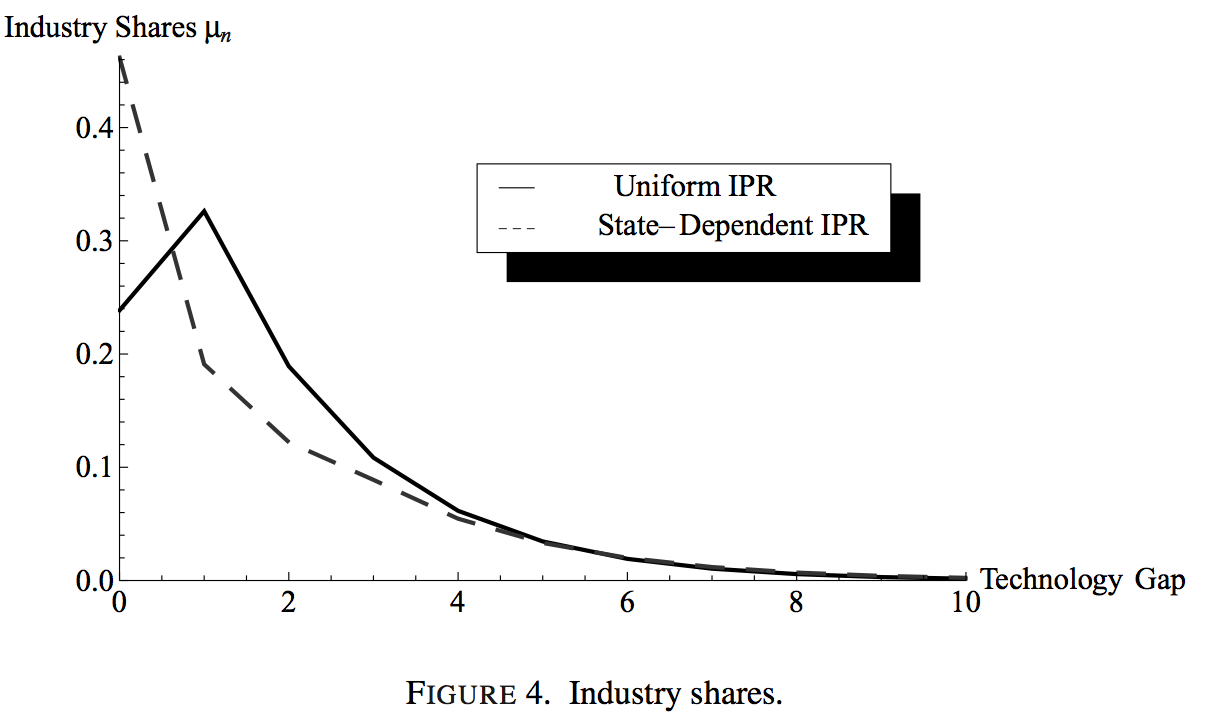
\includegraphics[scale=.28]{full_ipr_distbn.png}
    \label{fig:full_ipr_distbn}
  \end{center}
\end{frame}


\subsection{Software}
\label{sub:software}

% \begin{frame}[t]\frametitle{Software and Open Source}
%   \begin{itemize}
%     \item<+-> 
%   \end{itemize}
% \end{frame}
\subsection{Conclusion}
\label{sub:conclusion}

\begin{frame}[t]\frametitle{Summary}
  \begin{itemize}
    \item<+-> State-Dependent patent policy to motive all producers to innovate.
    \item<+-> Found that stronger protection should be given to those further ahead.
  \end{itemize}  
\end{frame}

% TODO: Add comparison frame.
\begin{frame}[t]\frametitle{Comparision}
    


\end{frame}

\begin{frame}[t]\frametitle{Conclusion}
  \begin{itemize}

    \item 
\includegraphics[scale=.025]{octocat.jpg} In the open source spirit: https://github.com/TomAugspurger/software

  \end{itemize}    
\end{frame}

\end{document}
